\documentclass[tikz,border=2mm]{standalone}
\usepackage{graphicx}
\usepackage{tikz}
\definecolor{ink}{HTML}{263238}
\begin{document}
\begin{tikzpicture}[font=\sffamily]
\node[anchor=south west,inner sep=0] (t1) at (0,5.92) {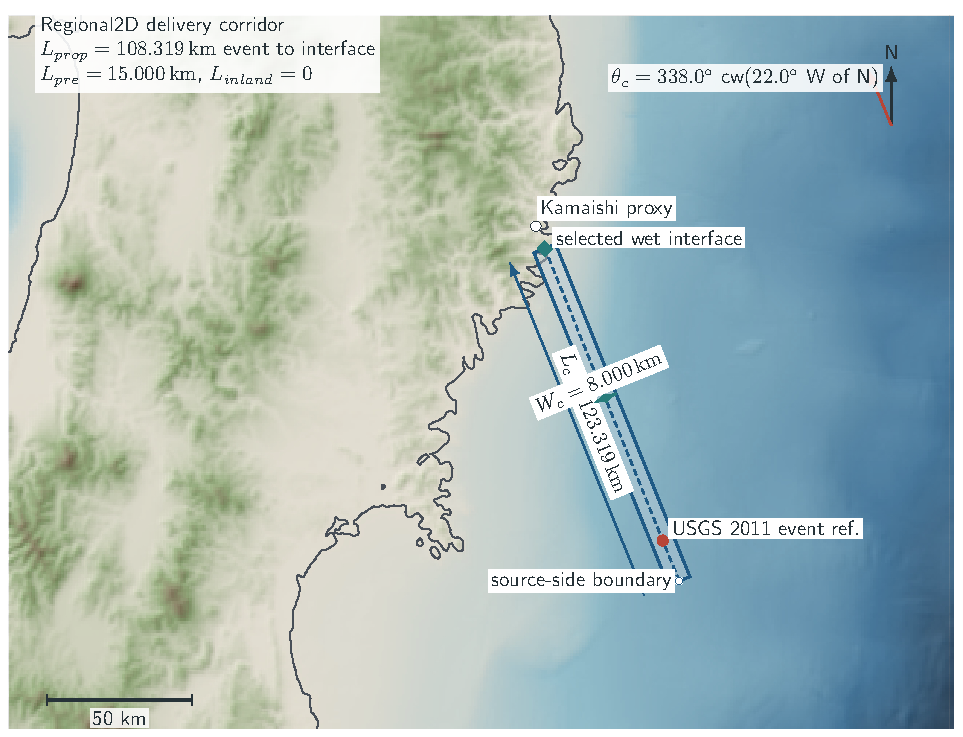
\includegraphics[width=8.9cm]{figure_T1_tohoku_kamaishi_domain.pdf}};
\node[anchor=south west,inner sep=0] (t3) at (9.15,5.92) {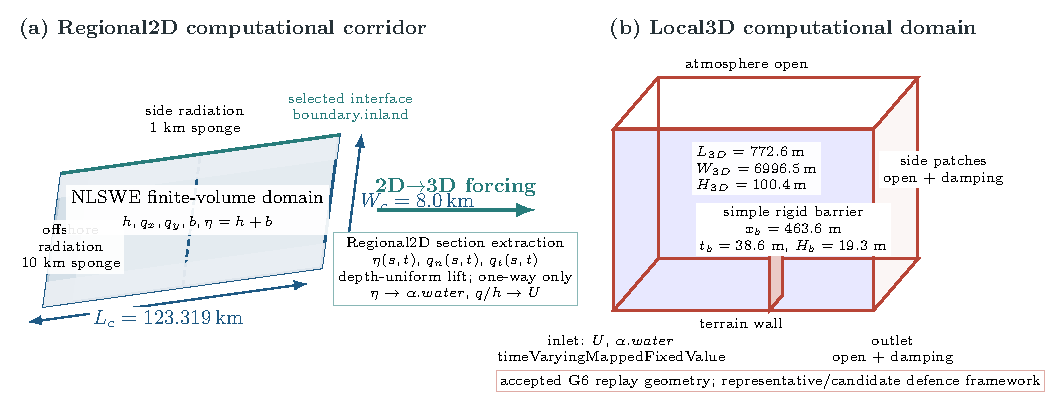
\includegraphics[width=14.65cm]{figure_T3_computational_domains.pdf}};
\node[anchor=south west,inner sep=0] (t2) at (0,0) {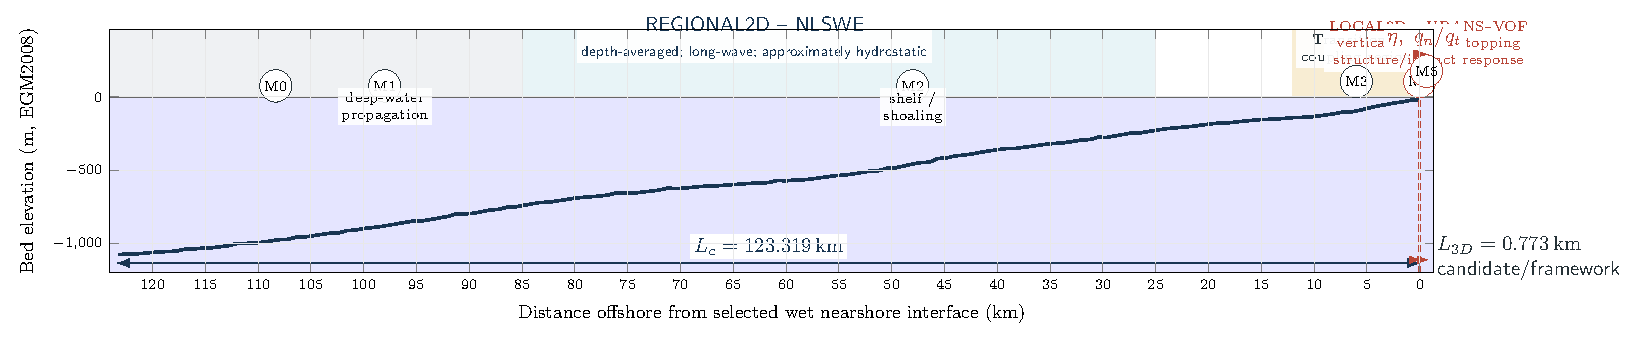
\includegraphics[width=23.80cm]{figure_T2_longitudinal_hybrid_corridor.pdf}};
\node[anchor=north west,fill=white,fill opacity=0.92,text opacity=1,inner sep=1.5pt,font=\bfseries,text=ink] at (0.10,14.38) {(a) geographic corridor};
\node[anchor=north west,fill=white,fill opacity=0.92,text opacity=1,inner sep=1.5pt,font=\bfseries,text=ink] at (9.25,14.38) {(b) computational domains};
\node[anchor=north west,fill=white,fill opacity=0.92,text opacity=1,inner sep=1.5pt,font=\bfseries,text=ink] at (0.10,5.78) {(c) longitudinal 2D$\rightarrow$3D corridor};
\node[anchor=south east,fill=white,fill opacity=0.9,text opacity=1,inner sep=1.6pt,font=\scriptsize,text=ink] at (23.72,0.10) {R19 composite preview: POSTER\_CANDIDATE};
\end{tikzpicture}
\end{document}
